\chapter{Descripción del Proyecto}\label{cap:01introduccion}

Este primer capítulo del Trabajo Fin de Grado (TFG) se divide en cinco secciones: \ref{sec:01intro} Introducción, \ref{sec:01Contexto} Marco contextual, \ref{sec:01EstadoArte} Estado del Arte, \ref{sec:01Motivacion} Motivación y \ref{sec:01estructura} Estructura de la memoria.

\section{Introducción} \label{sec:01intro}

Este proyecto se desarrolla en el marco contextual del auge de la Sanidad 4.0, consecuencia de la aplicación de las nuevas tecnologías de la Industria 4.0 en el sector sanitario. Es importantísimo conocer las características de este marco contextual porque son las que definen las nuevas necesidades en el tratamiento de la información sanitaria y dan sentido a la solución que ofrece el TFG.

En las siguientes secciones se presenta el contexto téorico del problema y la solución que aporta la organización Observational Health Data Science and Informatics (OHDSI), que es la que se emplea en este trabajo para satisfacer las necesidades descritas. Además, en el estado del arte se presentan soluciones alternativas que se están llevando a cabo de forma global y europea.

Posteriormente, se presenta la motivación personal de la alumna para realizar el trabajo y la colaboración con el Hospital Universitario Virgen del Rocío en esta labor. Para acabar con se expone brevemente la estructura y los contenidos que se tratan en esta memoria del proyecto y anexos.


\section{Marco contextual} \label{sec:01Contexto} 
%Intención: dar a conocer al lector los aspectos y características fundamentales del panorama sanitario y tecnológico actual, necesario para comprender en profundidad el trabajo.

El marco contextual de la problemática actual se encuentra influenciada por el surgimiento de la Industria 4.0 y las nuevas tecnologías que la acompañan, así como por su impacto significativo y transformador en el sector sanitario que ha generado nuevas necesidades a nivel mundial y europeo, más concretamente en el tratamiento de la información sanitaria. En este ámbito, la organización OHDSI se levanta como una solución innovadora y potente para paliar las necesidades de la industria.
%Estos desafíos han desembocado en Sevilla para formar parte del tópico trascendental de este trabajo.

\begin{figure}[H]
    \centering
    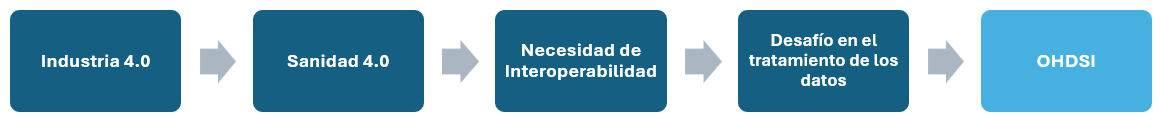
\includegraphics[width=0.90\textwidth]{figures/esquemaMarcoContextual.png}
    \caption{Esquema de contenidos de la sección}
    \label{fig:esquemaMarcoContextual}
\end{figure}


\subsubsection{Industria 4.0 y nuevas tecnologías}

La Industria 4.0, o cuarta revolución industrial, fue un concepto concebido por el gobierno alemán en noviembre de 2011 como una estrategia tecnológica para abordar el crecimiento industrial proyectado para 2020.
%Su uso internacional se popularizó en abril de 2013 durante la feria industrial de Hannover \textit{Hannover Messe}).
Este concepto representa la cuarta fase de la industrialización, sucediendo a la mecanización, electrificación e informatización, y destaca la integración digital de tecnologías avanzadas \cite{lasi2014industry}.

Se centra principalmente en la digitalización y la necesaria convergencia entre los sistemas físicos y cibernéticos (\textit{Cyber-Physical Systems, CPS}). Esta integración se busca a través de nuevas tecnologías de la información y telecomunicación (TICs), como el internet de las cosas (\textit{Internet of Things, IoT}), la generación y análisis de datos masivos (\textit{Big Data \& Big Data Analytics}), la computación en la nube (\textit{Cloud Computing}) y el auge de la Inteligencia Artificial (IA) \cite{lasi2014industry, chen2020times, tortorella2020healthcare}

\subsubsection{Características de la Sanidad 4.0}

La integración de los principios y tecnologías de la Industria 4.0 en el sector sanitario originó el concepto de Salud o Sanidad 4.0 (\textit{Healthcare 4.0}) \cite{tortorella2020healthcare, tortorella2021impacts}.  %
%En este contexto, este nuevo término se presenta como un complejo desafío  destinado a abordar los nuevos escenarios generados por la creciente demanda de dispositivos y sistemas médicos más eficaces y alineados con las nuevas TICs y los avances ininterrumpidos en ciencias como la biotecnología y la ingeniería genética. \cite{martin2021ehealth}. 
Esto origina un nuevo paradigma del que se destacan tres  características principales: la provisión continua de cuidado sanitario, la orientación de la medicina hacia el paciente y la prevención y predicción de enfermedades.


%Provisión continua de cuidado sanitario - Telemedicina, salud digital

\begin{itemize}

\item \textbf{Cuidado sanitario continuo (\textit{continuum of care})}. Gracias a tecnologías TIC y el IoT, la sociedad está altamente conectada, lo que ha impulsado el desarrollo de la telemedicina y la e-Salud, especialmente a raíz de la pandemia del COVID-19 \cite{martin2021ehealth}. Se han desarrollado numerosos dispositivos portátiles (\textit{wearable devices}), como pulseras y relojes inteligentes, para monitorear a los pacientes tanto dentro como fuera del hospital. Además estos dispositivos generan grandes cantidades de datos médicos que se combinan con registros clínicos para formar los llamados 'Datos del mundo real' \textit{(Real World Data, RWD)} \cite{kouroubali2019new}. 

La gran variedad en cuanto a la estructura y finalidad con la que se recopilan estos datos representan un desafío significativo en el tratamiento de la información clínica. La organización OHDSI pondrá fin a este desafío mediante la estandarización de las bases de datos RWD con un mismo fin: la invesigación observacional.

%\item \textbf{Provisión continua de cuidado sanitario}. La provisión continua del cuidado sanitario se basa en el cuidado continuo (\textit{continuum of care}) \cite{kouroubali2019new}. Gracias a las nuevas tecnologías de la Industria 4.0, mayoritariamente a las TICs y al IoT, la sociedad se encuentra estrechamente comunicada de forma prácticamente ininterrumpida. En el ámbito sanitario, a raíz de la pandemia del COVID-19 ha habido un creciente auge en el desarrollo de la telemedicina y la salud digital (\textit{e-Health}) \cite{martin2021ehealth} con el fin de monitorear al paciente dentro y fuera del complejo hospitalario. Para ello se ha potenciado el desarrollo de programas informáticos y dispositivos portátiles o \textit{wearables} de monitoreo de actividad como pulseras, relojes, sensores corporales, implantes inteligentes... Estos dispositivos generan enormes cantidades de datos médicos que junto a los registros clínicos de los hospitales generan una amplísima variedad de datos de pacientes reales. A estos conjuntos de datos se les denomina 'Datos del mundo real' (\textit{Real World Data}) y presentan un gran desafío actual en el tratamiento de los datos clínicos debido a su naturaleza de distintas índoles y que, además, cada organización recoge con distintos propósitos y estructura, lo que conlleva que frecuentemente se presenten grandísimas cantidades de datos inconsistentes, incoherentes o inaccesibles entre sí, produciéndose registros electrónicos de salud muy extensos y dispares. \cite{kouroubali2019new}.

%Patient-centred - Modelos de datos más amplios. Medicina de precisión.


\item \textbf{Centrada en el paciente}. Esta perspectiva enfatiza al paciente como el eje central de la atención sanitaria \cite{tortorella2020healthcare}. Con el avance de la medicina de precisión y el seguimiento remoto de la actividad diaria, la atención médica se vuelve cada vez más personalizada \cite{ruiz2023inteligencia}. La Unión Europea promueve esta orientación, exigiendo una reestructuración del sistema sanitario para que el paciente sea el principal beneficiario, evaluador y centro de los servicios de salud digital \cite{ntafi2022legal, katehakis2019framework}. Esto implica la implementación de sistemas informáticos que administren el historial clínico electrónico (HCE) completo de cada individuo, incluyendo observaciones de datos médicos, farmacéuticos y otros relevantes.

De esta forma, OHDSI presenta un modelo de datos lógico en el que el paciente es el núcleo central y alrededor de él se recoge información interseccional muy diversa, como medicamentos, procedimientos clínicos, etc.

%\item \textbf{Medicina centrada en el paciente}. La orientación de la medicina hacia el paciente se refiere a la priorización del paciente como objeto central de la provisión de salud  \cite{tortorella2020healthcare}. La atención sanitaria cada vez es más específica para cada individuo, gracias al seguimiento remoto de su actividad diaria y al auge de la medicina de precisión \cite{ruiz2023inteligencia}. La posición del foco de la salud en el paciente, fomentado por la Unión Europea,  implica reestructurar el sistema sanitario alrededor del mismo, pues el paciente debe ser el cliente final, juez y recibidor de todos los servicios y aplicaciones de la salud digital \cite{ntafi2022legal} \cite{katehakis2019framework}. En términos informáticos esto implica la reconfiguración de los sistemas médicos de modo que se recoja de manera central para cada individuo su historial clínico electrónico (HCE) completo, que incluya tanto datos médicos, como farmaceúticos y otros datos de interés.  

 %privacidad de datos, espacio de datos internacional, consentimiento en el uso secundario, acceso a los hce...

%Preventiva y predictiva - Herramientas de big data, IA

\item \textbf{Preventiva y predictiva}. Esta característica implica un enfoque proactivo en la salud en lugar de uno reactivo. La medicina se orienta hacia la prevención de enfermedades, utilizando análisis detallados del historial clínico del paciente y técnicas de aprendizaje automático (\textit{Machine Learning, ML}) para predecir y prevenir enfermedades antes de su aparición \cite{ruiz2023inteligencia}. Se emplean algoritmos avanzados de inteligencia artificial y aprendizaje automático, así como herramientas sofisticadas de análisis de datos, para abordar este desafío complejo y evolucionar hacia una atención médica más preventiva y predictiva.

La organización OHDSI presenta técnicas de ML embebidas en su herramienta de análisis por excelencia, ATLAS, que serán utilizadas en la reproducción del estudio al final del TFG.

%\item \textbf{Preventiva y predictiva}. La última característica es que sea preventiva y predictiva en lugar de meramente reactiva. Esto quiere que decir, que a diferencia del enfoque tradicional en el que la medicina es curativa, se debe transicionar hacia la provisión de salud de manera previa a la aparición de una enfermedad, de modo que esta pueda ser (i) predecida a través del análisis del HCE del paciente y/o exhaustivos análisis de precisión, y (ii) prevenida a través de monitorearización y provisión de tratamientos preventivos en el cuidado continuo de la salud \cite{ruiz2023inteligencia}. En esta línea el análisis del historial clínico de un paciente genera un desafío muy complejo y la prevención y la predicción se alcanza gracias al constante desarrollo de técnicas y algoritmos cada vez más sofisticados de inteligencia artificial y aprendizaje automático y herramientas cada vez más poderosas de ciencia y análisis de datos.
\end{itemize}

\subsubsection{Necesidad de interoperabilidad}

%Por último, la interoperabilidad entre sistemas y datos es el objetivo final de la revolución industrial, tecnológica y sanitaria actual. La necesidad de interoperabilidad es una realidad a la que se enfrentan todos los sectores y sistemas de información de las organizaciones públicas y privadas. La Comisión Europe identificó esta necesidad ya a principios de siglo \cite{CEU1999ida} y durante los años ha ido adquiriendo cada vez mayor relevancia. 

La interoperabilidad entre sistemas y datos es el objetivo principal de la actual revolución industrial, tecnológica y sanitaria. Esta necesidad es fundamental en todos los sectores y sistemas de información de organizaciones públicas y privadas, y ha sido reconocida por la Comisión Europea desde principios de siglo \cite{CEU1999ida}. En 2013, el IEEE definió la interoperabilidad como "la habilidad de los sistemas de intercambiar información y utilizarla de forma efectiva". 

Actualmente, el nuevo Marco de Interoperabilidad Europea (\textit{new EIF}, 2017) se encarga de ofrecer recomendaciones para mejorar la calidad de los servicios públicos europeos en términos de interoperabilidad, ya que se considera que "la falta de interoperabilidad es el mayor obstáculo para progresar" \cite{kouroubali2019new}. Aunque la clasificación de los tipos de interoperabilidad aún es confusa y no existe una única clasificación concreta \cite{santos2021interoperability}, la literatura coincide generalmente en tres tipos de interoperabilidad:

%En 2013, el IEEE definió el concepto de interoperabilidad como "la habilidad de los sistemas de intercambiar información y utilizar dicha información intercambiada de forma efectiva". Actualmente, el nuevo Marco de Interoperabilidad Europea (\textit{new EIF}, 2017) es el órgano encargado de ofrecer recomendaciones, modelos y guianza a fin de mejorar la calidad de los servicios públicos europeos en cuanto a interopeabilidad, pues se dice que "la falta de interoperabilidad es el mayor obstáculo para progresar" \cite{kouroubali2019new}.

%La clasificación de los tipos de interoperabilidad aún es algo confusa y no se ha establecido una única clasificación concreta \cite{santos2021interoperability}. No obstante, parece que la literatura coincide en los tres siguientes tipos de interoperabilidad:

\begin{itemize}

    \item \textbf{Interoperabilidad semántica}. La implementación de estándares o estandarización consiste principalmente en establecer acuerdos entre las grandes organizaciones de la salud para definir marcos específicos a través de los que estructurar la información clínica de manera única, reduciendo el desorden y la disparidad de los datos y permitiendo el intercambio de mensajes entre sistemas pertenecientes a distintas organizaciones. 
    %La estandarización es un requisito fundamental para alcanzar la interoperabilidad \cite{katehakis2019framework}. 
    Además con los estándares nace también un concepto importante: el código abierto o \textit{Open Source} para facilitar el acceso libre a la información y permitir consensuar un estándar común.
   %Sin ir más lejos, HL7, la mayor de las organizaciones entre las anteriores comenzó ofreciendo sus servicios de manera privada hasta 2012, cuando se decidió a promover el código abierto liberando la mayor parte de su propiedad intelectual para que pudiera ser accesible de forma gratuita. Esto potenció y promovió la adopción de estándares y la consecuente interoperabilidad entre las organizaciones sanitarias \cite{berryman2013data}.

   En este caso, OHDSI aboga por la interoperabilidad semántica aportando un estándar de datos \textit{open-source} que utiliza la gran mayoría de los otros estándares utilizados hasta el momento, bajo la premisa ''adopta en vez de inventa'' (\textit{Adopt instead of build}).

    \item \textbf{Interoperabilidad técnica}. Este tipo de interoperabilidad pone el foco en la conectividad, comunicación y operación relacionadas con las entidades interactivas y los elementos de middleware. En cuanto a la autenticación y autorización, el uso de estándares técnicos, protocolos de comunicación y transporte, e interfaces entre componentes \cite{santos2021interoperability}. La capa técnica abarca las aplicaciones e infraestructuras que vinculan sistemas y servicios. Incluye especificaciones de interfaz, servicios de interconexión e integración de datos, presentación y intercambio de datos, y protocolos de comunicación segura \cite{leal2019interoperability}.

    Para la interoperabilidad técnica entre sus sistemas, la organización propone diversas formas de implementación de su ecosistema de herramientas, sin imponer una única tecnología sino permitiendo al usuario configurar el entorno que más conveniente le sea.
    
    \item \textbf{Interoperabilidad organizacional}. Este nivel se centra en la interoperabilidad inter e intra organizacional, en cuanto a la definición común de reglas de negocio, políticas y restricciones, alineación de procesos y las acciones necesarias para hacer que las organizaciones colaboren \cite{motta2019conceptual}. También se refiere a cómo los sistemas de los participantes alinean sus procesos, responsabilidades y expectativas para lograr objetivos acordados comúnmente.

    OHDSI no es solo una organización científica sino una \textit{red de colaboradores} en la que los integrantes comparten la misma misión, visión y valores, entre otras políticas.

\end{itemize}

\subsubsection{Desafíos en el tratamiento de los datos}


A pesar de las numerosas iniciativas a nivel global y europeo, la transición hacia la interoperabilidad y estandarización sigue siendo muy desafiante debido a la complejidad y sensibilidad de los sistemas de información en salud. El manejo de datos sanitarios requiere gestiones precisas con protocolos de ciberseguridad estrictos y leyes de privacidad y confidencialidad bien definidas, lo que dificulta su implementación coordinada en diferentes regiones.

Se presentan a continuación algunos de los desafíos en el tratamiento de los datos clínicos, identificados en el Foro de Seguridad y Protección de Datos organizado por la SEIS en 2024 \cite{SEIS2024tercera, SEIS2024octava}.

\begin{enumerate}[label=\roman*.]
    \item \textbf{Ciberseguridad del sistema}. La ciberseguridad de los datos clínicos representa un desafío crítico. El creciente auge de amenazas cibernéticas constantes, requiere de actualizaciones y mejoras en las medidas de protección de la información médica. Las instituciones de salud deben estar a la vanguardia en la implementación de tecnologías de seguridad robustas para salvaguardar la integridad y la confidencialidad de los datos.
    \item \textbf{Confidencialidad y privacidad}.   La confidencialidad y privacidad de los datos clínicos también conforma un desafío relevante. Garantizar que solo las partes autorizadas tengan acceso a la información médica de los pacientes requiere no solo de protocolos tecnológicos sólidos, sino también de una cultura organizacional comprometida con el cumplimiento de las regulaciones de protección de datos y la ética médica. Para ello, además se necesitan protocolos de anonimización y pseudoanonimización de las bases de datos, que garanticen la privacidad de la información personal de los pacientes.
    \item \textbf{El uso secundario}. El consentimiento para el uso secundario de datos clínicos es otro aspecto crucial a considerar. A medida que se exploran nuevas formas de aprovechar los datos para la investigación y la mejora de la atención médica, es fundamental asegurar que los pacientes comprendan y otorguen su consentimiento informado para cualquier uso adicional de su información médica, respetando siempre su autonomía y derechos individuales.
    \item \textbf{Infraestructura tecnológica}. Por último, la infraestructura tecnológica adecuada es un requisito fundamental para el manejo eficiente de los datos clínicos. La arquitectura de los datos cada vez es más compleja y requiere infraestructuras tecnológicas muy potentes y costosas. Además, la falta de interoperabilidad entre sistemas, la obsolescencia de la tecnología y las limitaciones presupuestarias pueden obstaculizar los esfuerzos para la prestación de servicios TIC de salud.
    
\end{enumerate}

\subsubsection{Propuesta de solución}

Por tanto, ante las necesidades y desafíos del complejo panorama sanitario actual, este Trabajo de Fin de Grado propone a la organización \textbf{Observational Health Data Science \& Informatics (OHDSI)} como la solución óptima a la interoperabilidad en estudios observacionales con datos de salud, a través del Modelo de Datos Común de OMOP y la herramienta de análisis de datos \textbf{ATLAS}. 

De esta forma el proyecto pretende demostrar la utilidad y los beneficios de extraer evidencia utilizando las herramietnas estandarizadas de OHDSI a través de la reproducción de un estudio clínico sobre los efectos adversos de la radioterapia en pacientes oncológicos, llevado a cabo por el Hospital Universitario Virgen del Rocío, pero utilizando ATLAS en vez de la metodología tradicional.

La relevancia de OHDSI a nivel europeo es innegable, en marzo de 2020, la red de datos y evidencia de la unión europea, EHDEN (European Health Evidence \& Data Network) comenzó a colaborar con OHDSI para poner fin a la disparidad de estándares presente en los distintos nodos de la unión europea y proporcionar un Modelo de Datos Común y un espacio de datos interoperable y estandarizado para todos. A partir de entonces OHDSI ha comenzado a ganar gran relevancia a través de su participación en proyectos europeos como DARWIN EU (\textit{Data Analysis and Real World Interrogation Network European Unión}, 2022) \cite{OHDSI2023Darwin} %para proporcionar evidencia del mundo real de toda Europa sobre enfermedades, poblaciones y los usos y rendimiento de medicamentos \cite{Darwin2023website}
o EUCAIM (\textit{EUropean Cancer Image}, 2023).%que pretende establecer una red federada interoperable de compartición de imágenes oncológicas \cite{Kalokyri2023Early}.

Además a nivel estatal, España conforma uno de los nodos de colaboración con OHDSI más grandes de Europa. %Muchas organizaciones a lo largo del territorio español ya están colaborando con el estándar de OHDSI como la Agencia Española de Medicamentos y Productos Sanitarios (AEMPS) o Quirónsalud entre otros \cite{ohdsiSpain}. 
y en Sevilla, especialmente, la colaboración con OHDSI la llevan a cabo el IBIS (Instituto de Biomedicina de Sevilla), la fundación FISEVI (Fundación para la Gestión de la Investigación en Salud en Sevilla) y los hospitales universitarios Virgen Macarena y Virgen del Rocío. Este último además es la sede del convenio de prácticas en empresa realizadas junto al TFG . %El pasado octubre de 2023 el hospital Macarena celebró el 'Innodata 2023' \cite{HUVM2023INNODATA}, un congreso nacional sobre investigación de datos en salud, en la que se presentó una ponencia que trató las herramientas y experiencias de OHDSI. 


\section{Estado del Arte} \label{sec:01EstadoArte} 
%Intención: cuáles son las inicitivas que hay actualmente en el sector y cuál es la presencia real de OHDSI en el mismo.

\textcolor{red}{Boceto de contenidos básicos. Más ideas???? Más temáticas?? Mayor extensión???}

%En Europa, en noviembre de 2018 se lanzó la Red Europea de Datos y Evidencia en Salud (\textit{European Health Data \& Evidence Network, EHDEN}) con el objetivo de ''abordar los desafíos actuales en la generación de conocimientos y evidencia a partir de datos clínicos del mundo real a escala, para ayudar a los pacientes, médicos, pagadores, reguladores, gobiernos y la industria'' \cite{ehden}.

Frente a todo lo expuesto, aún no existe un consenso entre las grandes potencias que establezca verdaderamente una solución única. En el ámbito del tratamiento de la información sanitaria, existen numerosas alternativas a OHDSI y organizaciones proveedoras de estándares y herramientas para paliar las necesidades y dificultades del sector. Aunque irónicamente la presencia de tantísimas alternativas diferentes es la principal dificultad para la interoperabilidad.

En el ámbito de la interoperabilidad semántica, algunos de los estándares más reconocidos y usados mundialmente son HL7 FHIR \textit{(Health Level Seven - Fast Health Interoperability Resources)}, HL7 CDA \textit{(Health Level Seven Clinical Document Architecture)}, DICOM \textit{(Digital Imaging and Communications in Medicine)}, SNOMED CT \textit{(Systematized Nomenclature of Medicine - Clinical Terms)}, IHE (Integrating the Healthcare Enterprise), openEHR (Open Electronic Health Record), LOINC (Logical Observation Identifiers Names and Codes), RxNorm (Prescription Norm) entre otros.

Además, solo en España, cada comunidad autónoma utiliza un sistema informático sanitario distinto, cuyos datos están estructurados de formas distintas. En Andalucía el sistema de información es DIRAYA. Otros ejemplos son: en Madrid, Historia Clínica Digital de Atención Primaria (HCDSAP); en Cataluña, Sistema de Información de Atención Primaria (SIAP); en la Comunidad Valenciana, Sistema de Información Poblacional de Atención Primaria (SIPAP), en Pais Vasco, Osabide; en Galicia, SERGAS; entre otros.

Por otro lado, en el ámbito de la interoperabilidad técnica las alternativas son muy dispares, desde aquellos que realizan análisis totalmente personalizados mediante scripts de código o el gran catálogo de software de procesamiento de datos actualmente disponible en el mercado. Los lenguages de programación que más usan los analistas de datos son Python, R y SQL, implementados en diferentes IDEs como JupyterLab o Jupyter Notebook para Pyhton, Rstudio para R o multitud de plataformas de bases de datos (Oracle, Postgre, BigQuery...). Por otra parte, los software de análisis más extendidos son son Tableau, Microsoft PowerBI, SAS, MatLab, Apache Spark, entre otras. 

La falta de un estandar común es objeto de investigación en todo el mundo, lo que da lugar a alianzas entre organizaciones y competiciones en proyectos que pretenden dar solución a este aspecto, como por ejemplo la Infraestructura de Servicios Digitales de eSalud (eHDSI) \cite{DHE2023eHDSI} %representa un hito crucial en el impulso de la interoperabilidad y la integración de los sistemas de información sanitaria en Europa. Este marco establece estándares y protocolos para facilitar el intercambio seguro y eficiente de datos de salud entre los Estados miembros de la Unión Europea, con el objetivo de mejorar la calidad de la atención médica y promover la movilidad de los pacientes en el espacio europeo de salud digital \cite{EU2023Servicios}. 
o el proyecto European Genomic Data Infrastructure (GDI) \cite{GDI2022GDI} que busca establecer una infraestructura unificada para gestionar y compartir datos genómicos en Europa.
%abordando desafíos de interoperabilidad y ética. Su objetivo es promover la colaboración y la innovación en genómica, posicionando a Europa como líder en el uso responsable de datos genómicos para mejorar la salud.

%También las empresas privadas.

%%---------------------------------------------------------------------------

\section{Motivación} \label{sec:01Motivacion}

%Mi motivación personal de entrar en el mundo del %análisis de datos clínicos utilizando  esta %herramienta prometedora..

La principal motivación para realizar este proyecto ha sido mi curiosidad e interés por el mundo de la ciencia de datos a lo largo de mis años de formación universitaria. El origen se sitúa en el primer año de carrera, allá por el 2020, cuando por primera vez oí hablar del análisis de datos clínicos como una disciplina emergente de gran interés a nivel laboral. A partir de este momento, continué investigando sobre todo lo relacionado a esta disciplicina y cuando en tercero de carrera tuve la oportunidad de realizar el programa de movilidad ERASMUS al Politecnico di Milano, no dudé en seleccionar el mayor número de asignaturas de Data Science que mi convenio de estudios me permitió. 

Este año de estudio en Milán confirmó que, lo que había nacido como una mera curiosidad, se había convertido en una pasión, por lo que a mi regreso del Erasmus me decidí a orientar mi carrera profesional y mi TFG hacia el mundo del análisis de datos clínicos, hasta el día de hoy en que este Trabajo Fin de Grado es escrito.

El Trabajo Fin de Grado ha sido realizado por mi, María del Valle Alonso de Caso Ortiz, alumna del grado de Ingeniería de la Salud por la Universidad de Sevilla (US), de la promoción 2020-2024 y bajo la tutela de D. Julián A. García García y Da. Maria J. Escalona Cuaresma, ambos pertenecientes al departamento de Lenguajes y Sistemas Informáticos de la Escuela Técnica Superior de Ingeniería Informática (ETSII) de la misma universidad. 

Además se ha realizado en conjunto con el Departamento de Innovación Tecnológica del Hospital Universitario Virgen del Rocío, mediante un convenio de prácticas curriculares de 337 horas, donde han ejercido la tutela D. Silvia Rodríguez Mejías y D. Carlos Luis Parra Calderón. 

De esta forma, también ha sido de gran importancia la motivación de mis profesores y tutores de la ETSII y compañeros del grupo científico del Departamento de Innovación Tecnológica del hospital, quienes confiando en mi me han apoyado, motivado y guiado durante mi formación sobre ATLAS y OHDSI y la informática clínica en general.

\section{Estructura de la memoria} \label{sec:01estructura}

La memoria se estructura en diez capítulos y dos anexos que contienen toda la información relevante.

La información propiamente sobre el proyecto se encuentra en los capítulos: \ref{cap:01introduccion} Descripción del Proyecto \ref{cap:02objetivos} Objetivos del Proyecto, \ref{cap:03gestión} Gestión del Proyecto y \ref{cap:04metodologia} Metodología.

A continuación, en \ref{cap:05EstudioPrevio} Marco Teórico, se recopila información relevante sobre la organización Observational Health Data Science and Informatics (OHDSI) y sus herramientas, prestando especial atención a ATLAS. Este capítulo en conjunto con \ref{cap:06requisitos} Documento de Requisitos y \ref{cap:07diseño} Entorno de Trabajo proveen un conocimiento teórico completo de las herramientas y análisis a tratar durante el proyecto. 

Por otra parte, en \ref{cap:08pruebas} Caso práctico se presenta un capítulo dedicado a la reproducción de un caso práctico de estudio utilizando ATLAS. 

Por último, los siguientes dos capítulos \ref{cap:09resultados} Resultados y \ref{cap:10conclusiones} Conclusiones, presentan una recopilación de resultados y conclusiones, respectivamente obtenidos al término del desarrollo del TFG. 

Adicionalmente, se adjuntan dos anexos. El anexo \ref{anexo:manual} consiste en una guía completa de Instalación, despliegue y configuración de Broadsea y el Anexo \ref{anexo:glosario}, se trata Glosario de Términos técnicos relevantes para la comprensión del trabajo. 

Por su naturaleza informática, este TFG se ha desarrollado paralelamente a un repositorio de github del proyecto \cite{vallealonsodc}, que ha servido como controlador de versiones y como administrador de archivos en la nube, permitiendo almacenar y compartir con el lector archivos relevantes del TFG, ya sean archivos necesarios para el despliegue de la herramienta, archivos producidos durante el análisis o los propios documentos en sí mismos.
